\documentclass[a4paper,11pt,notoc]{article}
\usepackage{jheppub}
\usepackage{ulem}
\usepackage{graphicx}


\newcommand{\Zmumuj}   {\mbox{${\mathrm Z}(\rightarrow\mu \mu$)+jets}}
\newcommand{\Zeej}   {\mbox{${\mathrm Z}(\rightarrow e e$)+jets}}
\newcommand{\Zllj}   {\mbox{${\mathrm Z}(\rightarrow l l$)+jets}}
\newcommand{\Zll}   {\mbox{${\mathrm Z}(\rightarrow l l$)}}
\newcommand{\ttbar}   {\mbox{${t\bar{t}}$}}
%\newcommand{\Zee}   {\mbox{${\mathrm Z}(\rightarrow e e$)}}
\newcommand{\Znunuj}   {\mbox{${\mathrm Z}(\rightarrow\nu \nu$)+jets}}
\newcommand{\Znunu}   {\mbox{${\mathrm Z}(\rightarrow\nu \nu$)}}
\newcommand{\Wlnuj}   {\mbox{${\mathrm W}(\rightarrow l\nu$)+jets}}
\newcommand{\Wlnu}   {\mbox{${\mathrm W}(\rightarrow l\nu$)}}
\newcommand{\Wenuj}   {\mbox{${\mathrm W}(\rightarrow e\nu$)+jets}}
\newcommand{\pt}{\ensuremath{\mathrm{p_T}}}
\newcommand{\ptZ}{\ensuremath{\mathrm{p_T^{Z}}}}
\newcommand{\met}{\ensuremath{\not\!\!E_T}}
%\newcommand{\Wenu}   {\mbox{${\mathrm W}(\rightarrow e\nu$)}}
\title{ Pushing the precision frontier at the LHC with V+jets}
%	{\Large \bf Proceedings for the workshop on 'Illuminating standard candles a the LHC: V+jets' held at Imperial College London on April 25th-26th}\\
%\end{center}
\author[d]{Ulla~Blumenschein,}
\author[b]{Shane~Breeze,}
\author[e]{Chiara~Debenedetti,}
\author[g]{Engin~Eren,}
\author[k]{Simona~Gargiulo,}
\author[b]{Nigel~Glover,}
\author[b]{Jonas~Lindert,}
\author[b]{Daniel~Maitre,}
\author[a]{Sarah~A.~Malik,}
\author[c]{Bjoern~Penning,}
\author[g]{Svenja~K.~Pflitsch,}
\author[f]{Darren~Price,}
\author[l]{Stefan~Richter,}
\author[h]{Marek~Schoenherr,}
\author[b]{Peter~Schichter,}
\author[j]{Paolo~Torrielli,}
\author[i]{Maria~Ubiali,}
\author[a]{Nicholas~Wardle,}
\author[a]{Angelo~G.~Zecchinelli}

\affiliation[a]{High Energy Physics Group, Blackett Laboratory, Imperial College, Prince Consort Road, London, SW7 2AZ, UK\ }
\affiliation[b]{Institute for Particle Physics Phenomenology, Durham University, Durham, DH1
 3LE, UK}
\affiliation[c]{Bristol University, HH Wills Physics Laboratory, Tyndall Avenue, Bristol, BS8 1TL, UK}
\affiliation[d]{Queen Mary University of London, Mile End Road, London, E1 4NS, UK}
\affiliation[e]{University of California Santa Cruz, 1156 High Street, Santa Cruz, California, US}
\affiliation[f]{The University of Manchester, Oxford Rd, Manchester, M13 9PL, UK}
\affiliation[g]{Deutsches Elektronen-Synchrotron DESY, Notkestraße 85, 22607 Hamburg, Germany}
\affiliation[h]{University of Zurich, Rämistrasse 71, CH-8006, Zürich, Switzerland}
\affiliation[i]{University of Cambridge, The Old Schools, Trinity Ln, Cambridge CB2 1TN, UK}
\affiliation[j]{Università di Torino, Via Giuseppe Verdi, 8, 10124 Torino, Italy}
\affiliation[k]{Albert Ludwigs University of Freiburg, Fahnenbergplatz, 79085 Freiburg im Breisgau, Germany}
\affiliation[l]{University College London, Gower St, Bloomsbury, London WC1E 6BT, UK}
\begin{document}
\maketitle
\flushbottom

\section{Motivation}
Processes in which a vector boson is produced in association with jet(s) in proton-proton collisions (V+jets) at the Large Hadron Collider are valuable probes of perturbative QCD. In addition they constrain Parton Distribution Functions and play a crucial role in the fits to PDFs. They are also dominant backgrounds in the search for physics beyond the Standard Model in models of Supersymmetry, Dark Matter and Higgs boson decays into invisible particles. In some channels such as jets plus missing transverse momentum, they can contribute up to 90\% of the total background. Increasing the sensitivity of these searches in Run 2 of the LHC relies critically on reducing the systematic uncertainties on the V+jets background processes. 

The LHC is now in its second phase of running (Run 2), colliding protons at the higher center of mass energy of 13 TeV and expecting to accumulate an order of magnitude more luminosity in Run 2 than has previously been studied. As the LHC enters an era of precision, this presents a tremendous opportunity to conduct measurements of V+jets processes in regions of phase space that were previously limited by statistics, such as the high transverse momentum region that is characteristic of the phase space probed by our searches. In parallel, developments in theoretical calculations means we have improved predictions and state of the art Monte Carlos becoming available, with the near term prospect of having automated NLO QCD and EWK corrections. 
Studying V+jets processes in regions of phase space that have previously not been studied extesnively due to poor statistics and also in corners of phase space such as the collinear W measurment and VBF production and also using V+jets as a tool to understand the splitting scales in the kT clustering of jets, allowing us to bettwe measure the transition between the hard and soft hadronic activity which are not directly probed by jet-based measurements. 


- Motivation
- Experimental overview of V+jet measurements
- Theoretical developments (developments in higher order calculations, Monte Carlo generators)
- Backgrounds to BSM searches
- Outcome/Wishlist

\section{Experimental overview of V+jet measurements}

\section{Summary of theoretical developments}
\subsection{Higher order QCD and EWK corrections}
Developments in calculation of higher order corrections and evaluation of theoretical uncertainties

The sources of theoretical uncertainties on these processes are principally from three main sources; (1) missing higher order corrections, (2) uncertainties in input parameters such as parton distributions, masses and couplings, and (3) uncertainties in the parton/hadron transition including the fragmentation which is modeled by the parton shower, the hadronisation and the underlying event. 
The theoretical uncertainties from missing higher order corrections can be improved by the inclusion of higher orders and the resummation of large logarithms, those on the input parameters are be improved by a better description of the benchmark processes(?) and on the parton-hadron transition by improving the matching/merging at higher orders and the estimation of non-perturbative effects. While NLO QCD is the current state of the art, there have been rapid development in the calculation of NNLO QCD with many results becoming available. The higher order corrections from NLO EW corrections are roughly similar in size to the NNLO QCD and become particularly important at high energies and when probing higher transverse momenta and near resonances. 
- NNLO QCD calculations are available for all V+jet processes. All the calculations are at the parton level and can compute fiducial cross-sections. However, the codes are complicated to use and typically require significant CPU resources. The NNLO calculations are emerging as the standard for high statistic benchmark processes like V+jets and show the anticipated features expected of this calculation, a reduced dependence on the renormalisation scale and hence a reduction in the scale uncertainty, stabilisation of the perturbative series, more partons in the final state so perturbation theory can start to reconstruct the shower, and will lead to improved PDFs, hence further reducing the theory uncertainty. 
Higher order electroweak corrections have become important at the large p$_{T}$, H${_T}$. 
The NNLO calculation normalised to the NNLO Drell-Yan cross-section significantly improves the agreement with data for the \ptZ distribution shown in Figure~\ref{fig:ptNNLO} with a sbstantially reduced scale uncertainty. The photon p$_T$ has also recently been calculated to NNLO, the comparison with the p$_{T}$ spectrum from ATLAS is shown in Figure~\ref{fig:ptNNLO}. While the shape of the distribution does not show a significant improvement with data compared to the NLOdescription, the theoretical uncertainty is significantly reduced. Combining the NNLO calculation with NLO EWK prediction describes the data much better, in particular in the high pT region where the higher order EWK corrections become dominant. 
NNLO calculations require regularization of infrared singularities that are present in phase spaces with different numbers of final state partons, different approaches are used to do this. 
EWK corrections generally arising from loop diagrams in which a virtual W or Z is exchanged , resulting in leading logarithms of the form log$^2(M_V/p_T)$. For gamma+jets the correction from NLO to NNLO is around 10\%. The NNLO/NLO k-factor is reasonably flat, with a slight increase at higher pT. Scale variation of 2-3\% for the NNLO prediction compared to 8-10\% for the NLO. Both predictions consistently below experimental data. The effects of electroweak corrections are inclued by rescaling the complete NNLO result by the change observed in the LO prediction when including one-loop electroweak effects. The overall agreement between data and prediction gets worse when including the electroweak corrections, but the normalised distribution shows that the shape is much better described with the inclusion of EWK corrections. At NNLO the scale variation and PDF uncertainty are roughly equal and give a few percent uncertainty. The PDF uncertainty is the largest uncertainty and gives 5\% at high photon transverse momentum, the total uncertainty then ranges from 4\% at low pT to 9\% at high pT of 1 TeV. 
\begin{figure}[t!]
\centering
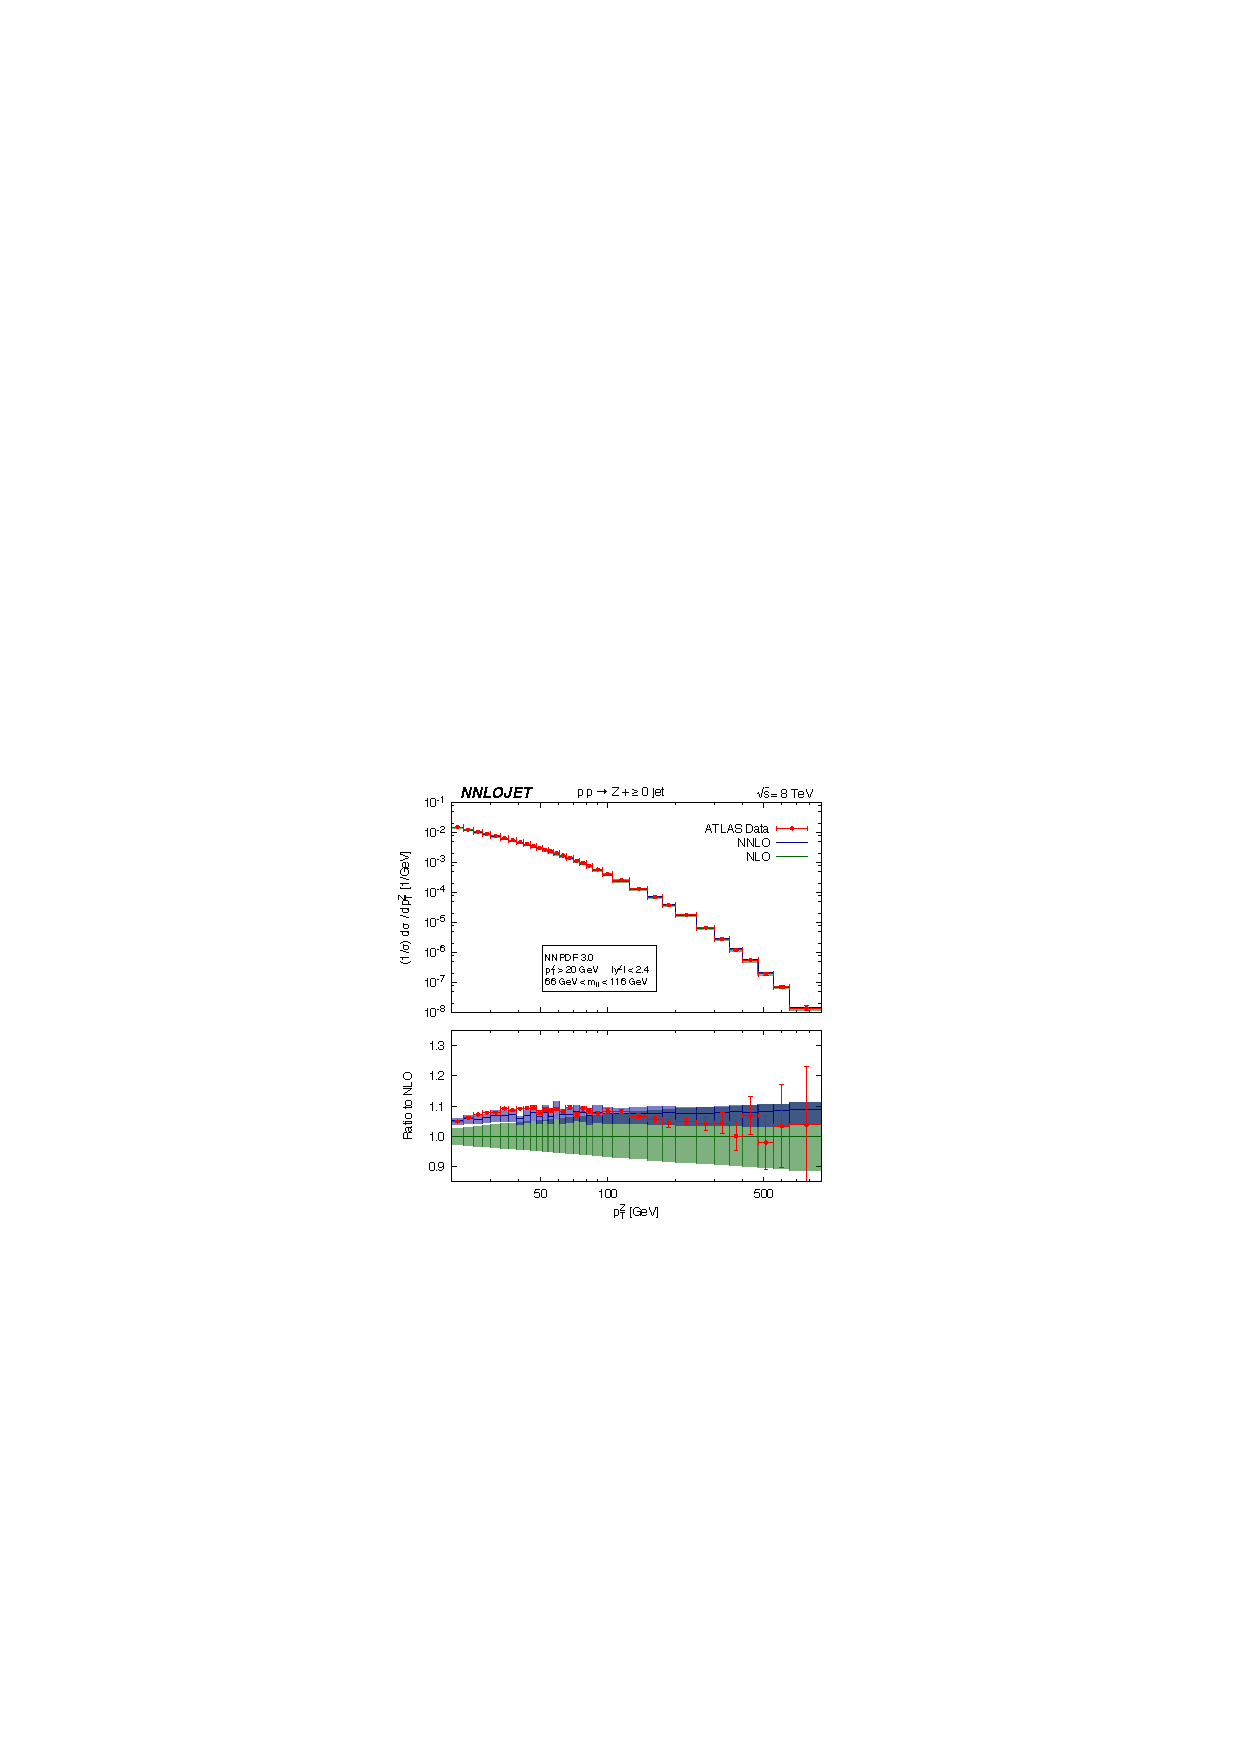
\includegraphics[width=0.495\columnwidth]{ptZNNLO.pdf} 
\caption{Comparison of the NNLO \ptZ distribution normalised by the NNLO Drell-Yan cross section with data from ATLAS.}
\label{fig:ptNNLO}
\end{figure}   

\begin{figure}[t!]
\centering
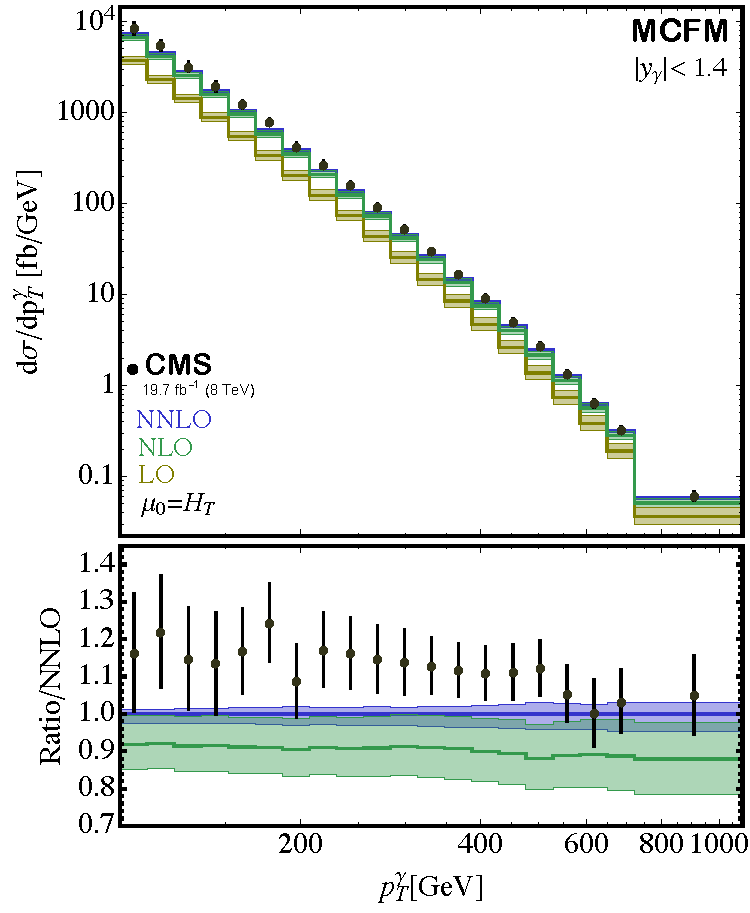
\includegraphics[width=0.495\columnwidth]{pt_gam.pdf} 
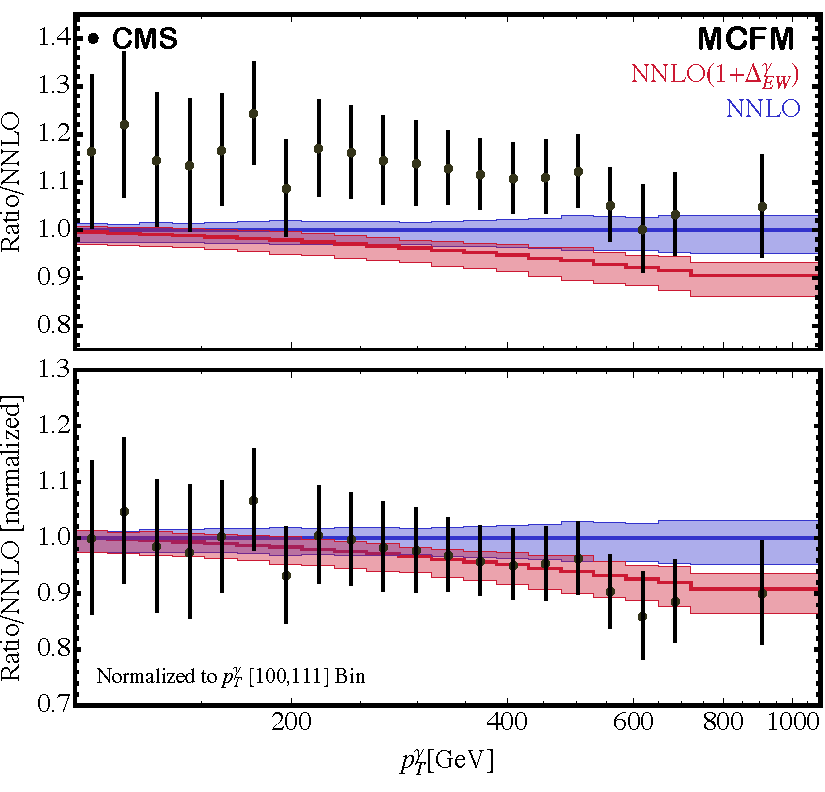
\includegraphics[width=0.495\columnwidth]{pt_gam_EW_norm.pdf} 
\caption{Comparison of the NNLO \ptZ distribution normalised by the NNLO Drell-Yan cross section with data from ATLAS.}
\label{fig:ptNNLO}
\end{figure}   

\begin{figure}[t!]
\centering
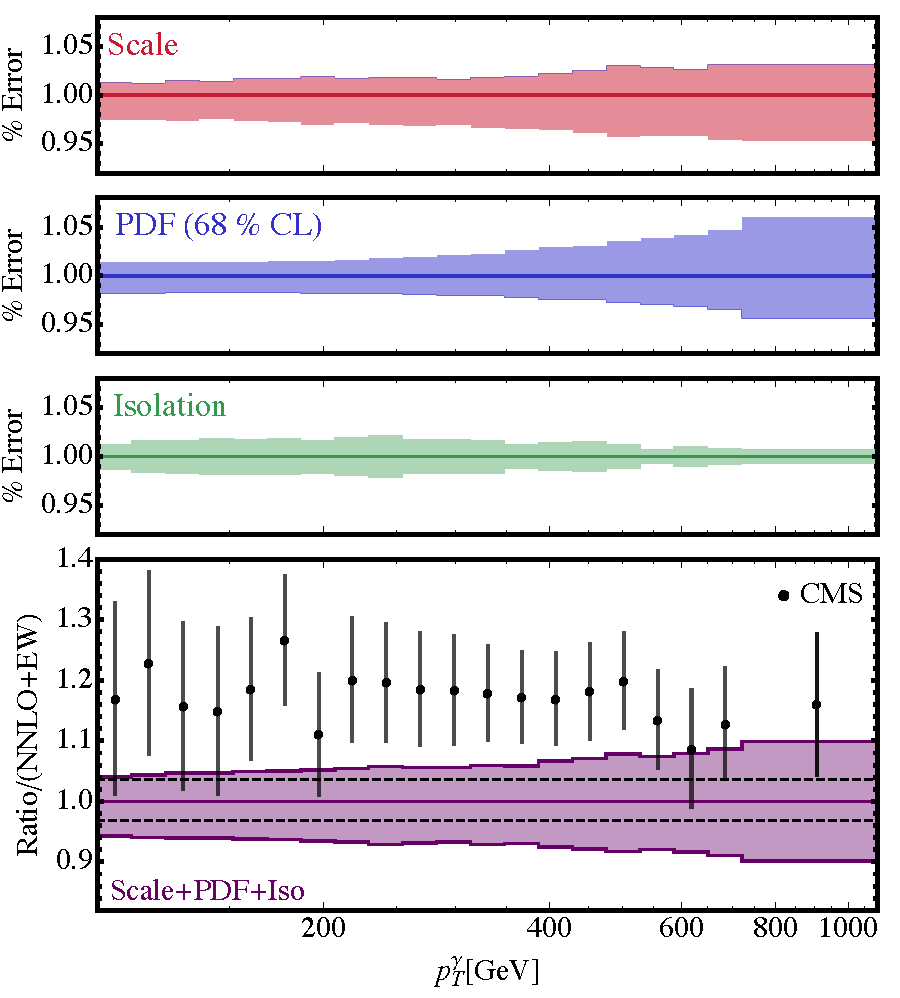
\includegraphics[width=0.495\columnwidth]{ptgam_uncert.pdf} 
\caption{Comparison of the NNLO \ptZ distribution normalised by the NNLO Drell-Yan cross section with data from ATLAS.}
\label{fig:ptNNLO}
\end{figure}   

\begin{figure}[t!]
\centering
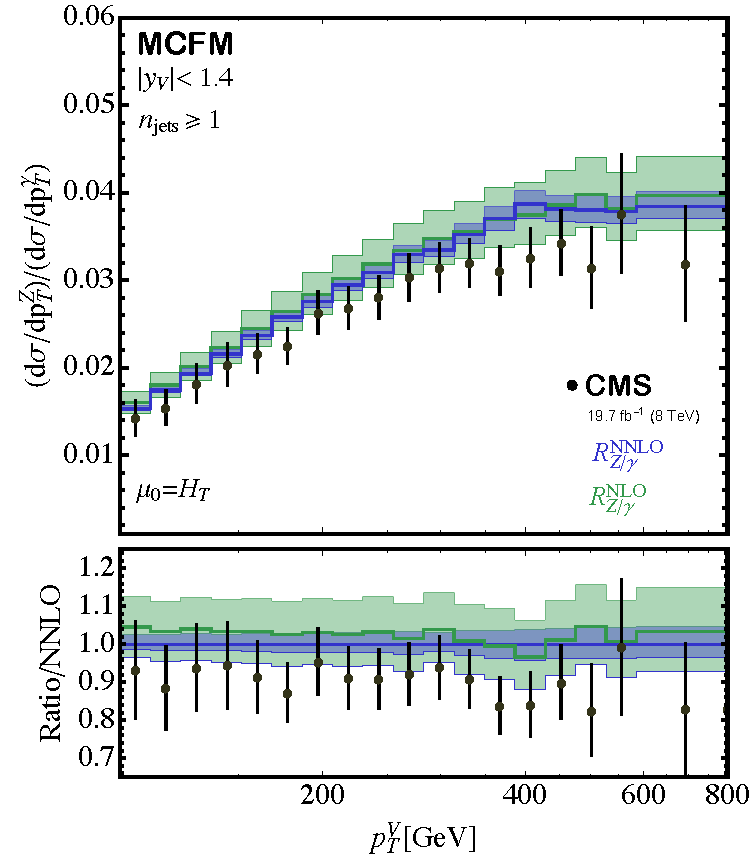
\includegraphics[width=0.495\columnwidth]{Zga_ratio_8TeV.pdf} 
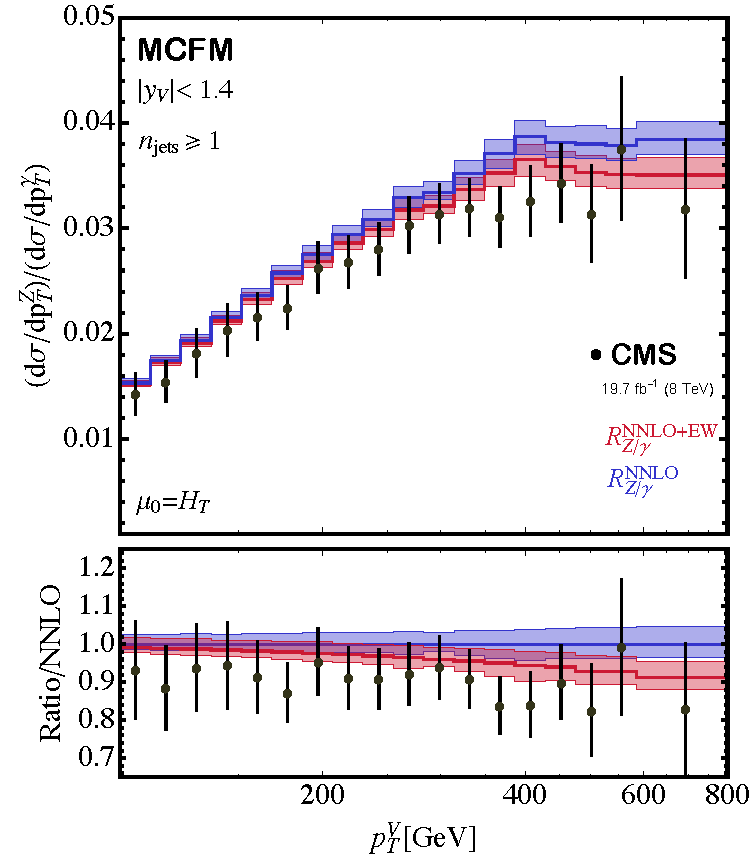
\includegraphics[width=0.495\columnwidth]{Zga_ratioEW_8TeV.pdf} 
\caption{Comparison of the NNLO \ptZ distribution normalised by the NNLO Drell-Yan cross section with data from ATLAS.}
\label{fig:ptNNLO}
\end{figure}   

\begin{figure}[t!]
\centering
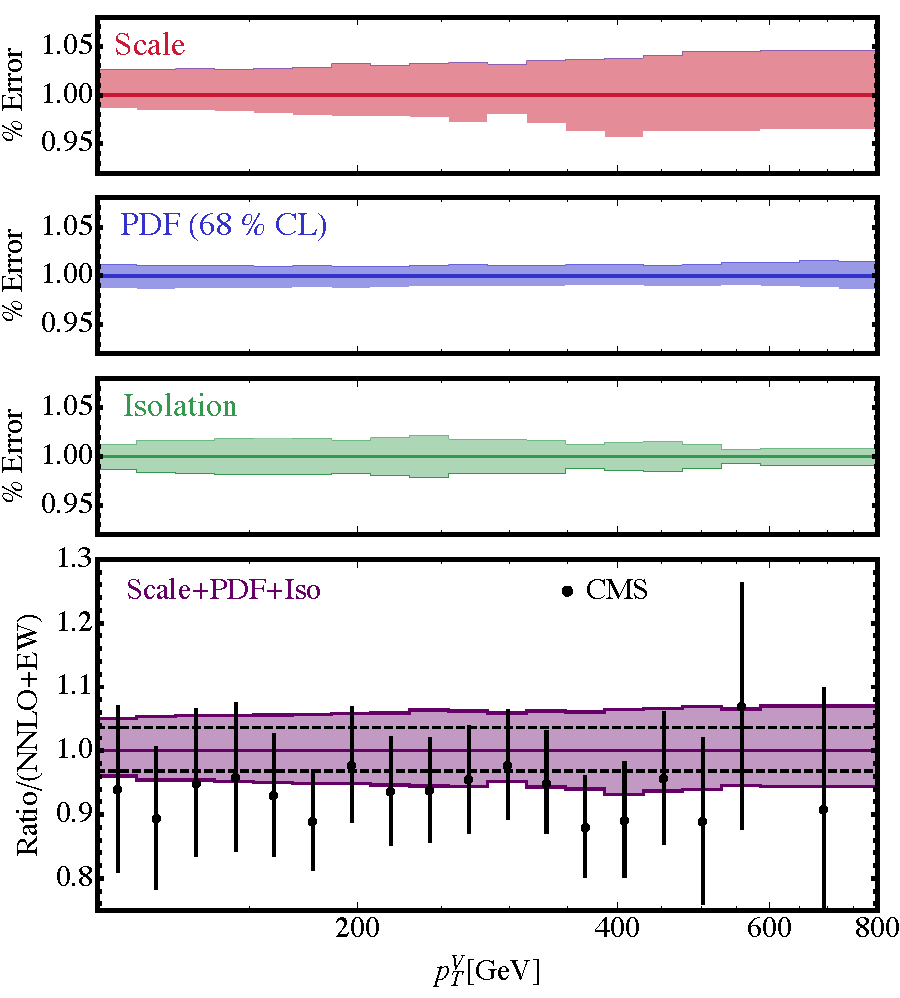
\includegraphics[width=0.495\columnwidth]{ptZga_uncert.pdf} 
\caption{Comparison of the NNLO \ptZ distribution normalised by the NNLO Drell-Yan cross section with data from ATLAS.}
\label{fig:ptNNLO}
\end{figure}   

The inclusive W+1jet production is important for calibrating the missing transverse momentum attributed to the neutrino. It has large NLO corrections of the order of 40\% owing to new partonic configurations from the soft/collinear W radiation from dijet events. The NNLO corrections are relatively small leading to a significant reduction in the scale uncertainty. Requiring only one jet eliminates the new configuratiosn and leads to more moderate NLO effects at the level of 20\%. The QCD perturbative expansion displays good convergence after inclusion of the NNLO corrections.  

The fiducial cross sections are shown at 13 TeV for the inclusive and exclusive 1-jet bin in Table~\ref{tab:Wjet}. The NLO correction increases the LO result by 42\% for the inclusive case and by 16\% for the exclusive bin, while including the NNLO corrections increases the inclusive cross section by 3\% while reducing the exclusive 1-jet cross section by 4\%. The cause of these different corrections for the inclusive and exclusive case is due to jet veto logarithms which can have a significant impact on fixed-order cross sections in exclusive jet bins. The pTW distribution is shown in Figure. The NLO corrections above ptW ~ 200 GeV are at a maximum of 60\% and then slowly decrease to 40\% at a ptW of 1 TeV with an uncertainty from scale variation of 20\%, while the NNLO corrections are ~10\% at ptW of 200 GeV and remain roughly constant out to high pT, with an uncertainty from scale variation of a few percent. The corrections have a very different impact on the exclusive jet distribution owing to the jet veto logarithms with increase with the transverse momentum. The NLO correction is 0.9 at ptW of 200 GeV and decreases to 0.3 for ptW of 800 GeV. The NNLO correction is roughly constant from ptW of ~ 50 GeV at 0.9. For the HT distribution, there is a large K-factor for the NLO, the NNLO corrections are much smaller than the NLO corrections, the NLO corrections grow to 75\% when the HT is $>$ 1 Tev, with a residual scale dependence of $\pm 15\%$. Work is needed to compare this with a merged W+jets sample. At NLO there are configurations containing 2 hard jets and a soft/collinear W boson that are logarithmically enhanced. These cannot occur at LO since the W boson must balance in the transverse plane against the single jet that appears. the NLO corrections are large bu the QCD pertubative expansion stabilises when the NNLO corrections are included. 

\begin{table}[h!]
\centering
\begin{tabular}{|c|ccccc|} \hline
  & $\sigma_{\mathrm {LO}}$ (pb) & $\sigma_{\mathrm {LO}}$ (pb) & $\sigma_{\mathrm {LO}}$ (pb) & $\mathrm {K_{NLO}}$ & $\mathrm {K_{NNLO}}$ \\ \hline 
inclusive & $773.7^{+33.7}_{-36.8}$ & $1099.3^{+57.8}_{-44.6}$ & $1130.2^{+5.2}_{-8.7}$ & 1.42 & 1.03 \\
exclusive & $773.7^{+33.7}_{-36.8}$ & $895.7^{+16.0}_{-11.6}$ & $863.2^{+10.5}_{-13.0}$ & 1.16 & 0.96 \\ \hline
\label{tab:Wjet}
\end{tabular}
\end{table}

\begin{figure}[t!]
\centering
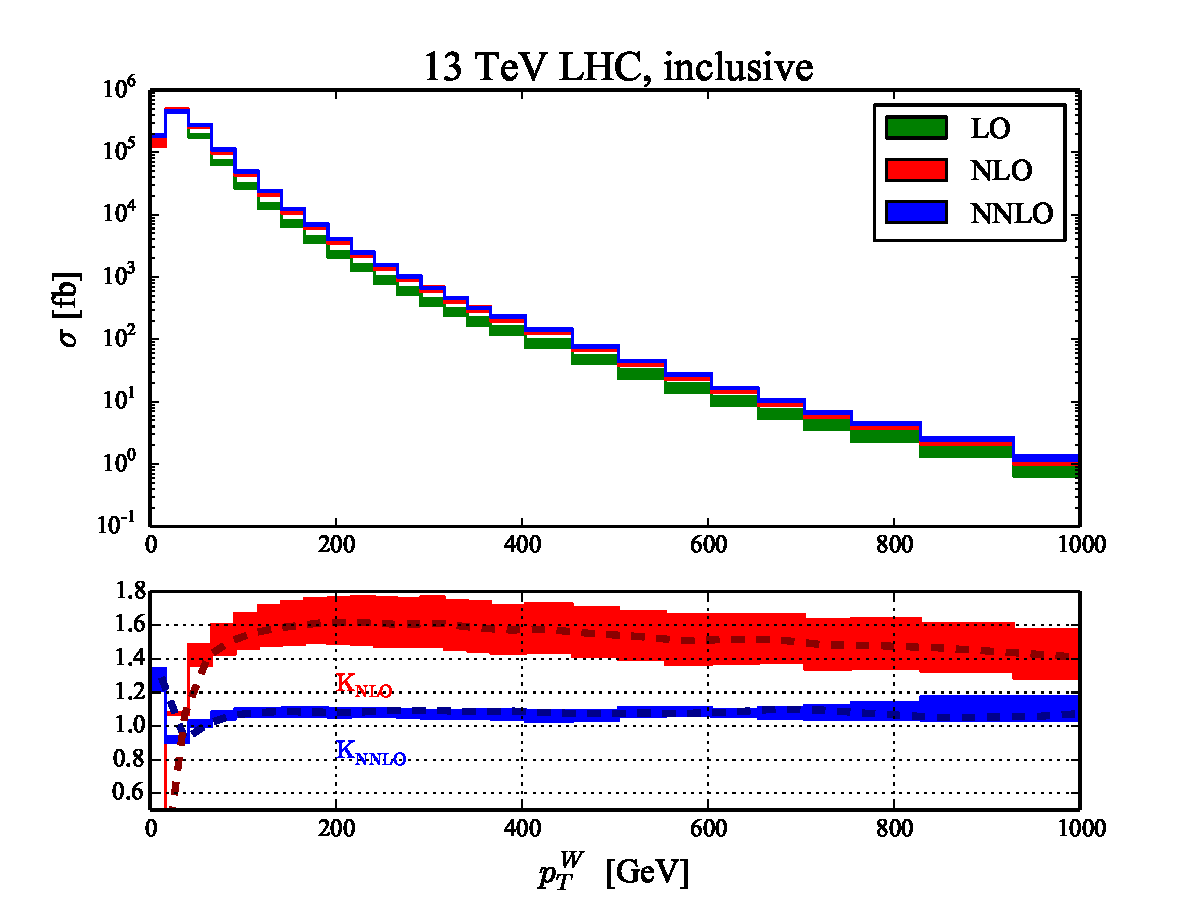
\includegraphics[width=0.495\columnwidth]{pTW_13TeV_incl.pdf} 
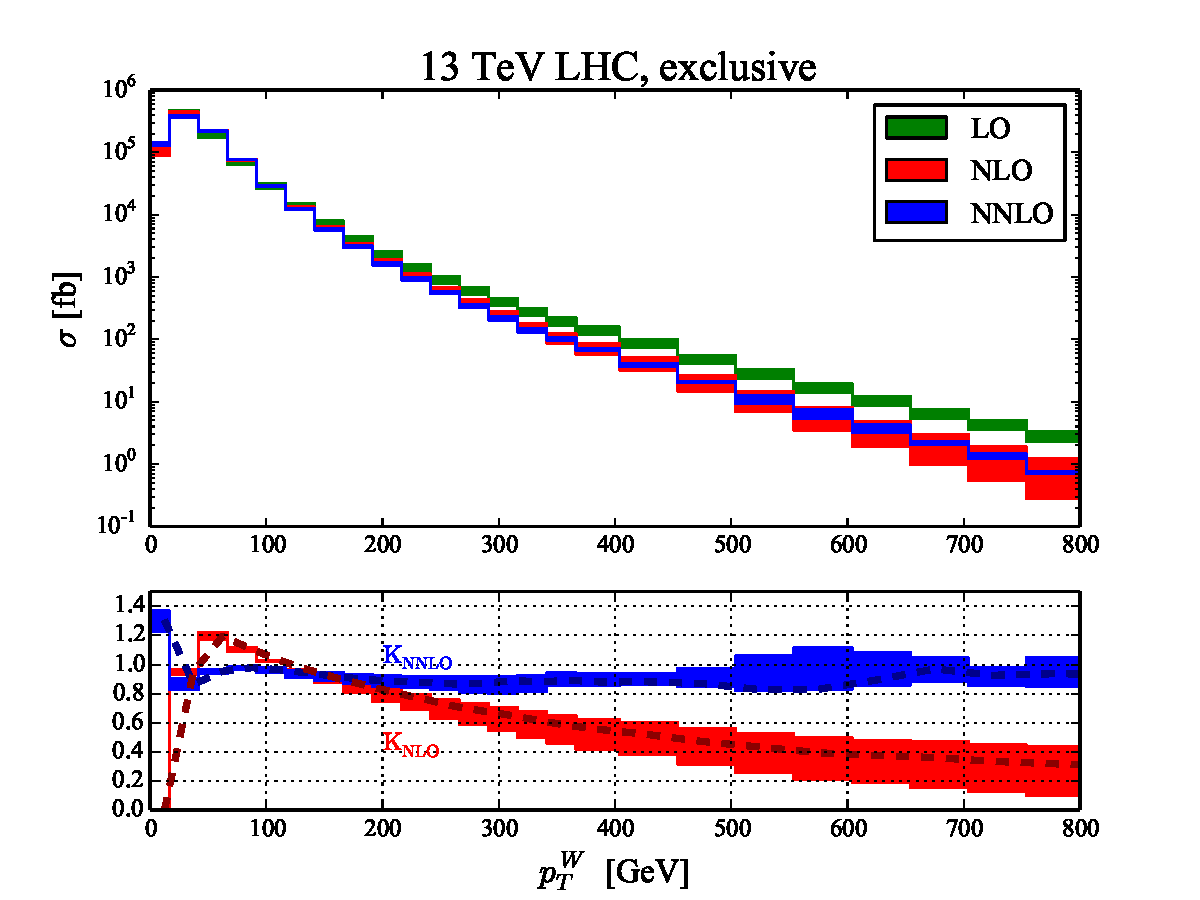
\includegraphics[width=0.495\columnwidth]{pTW_13TeV_excl.pdf} 
\caption{Comparison of the NNLO \ptZ distribution normalised by the NNLO Drell-Yan cross section with data from ATLAS.}
\label{fig:ptNNLO}
\end{figure}   


\begin{figure}[t!]
\centering
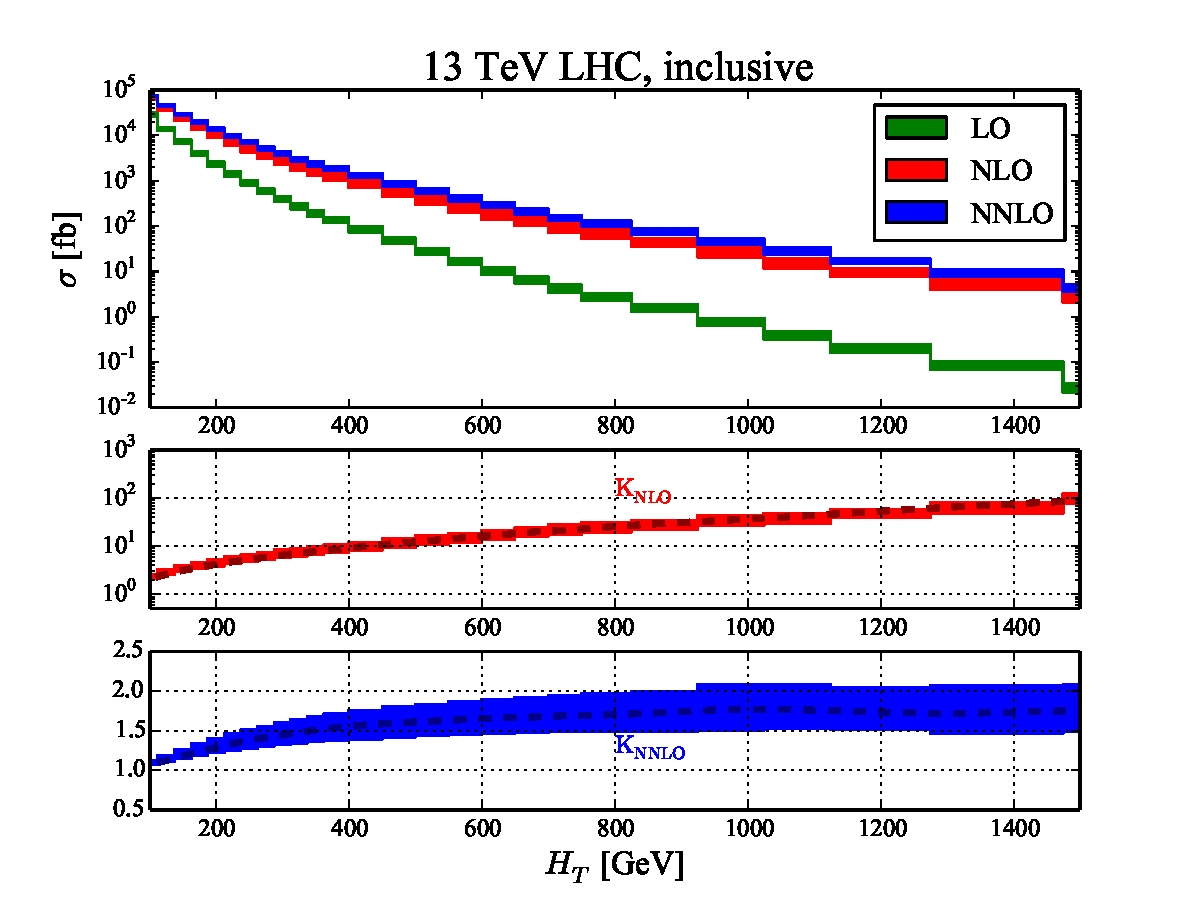
\includegraphics[width=0.495\columnwidth]{HT_13TeV_incl.pdf} 
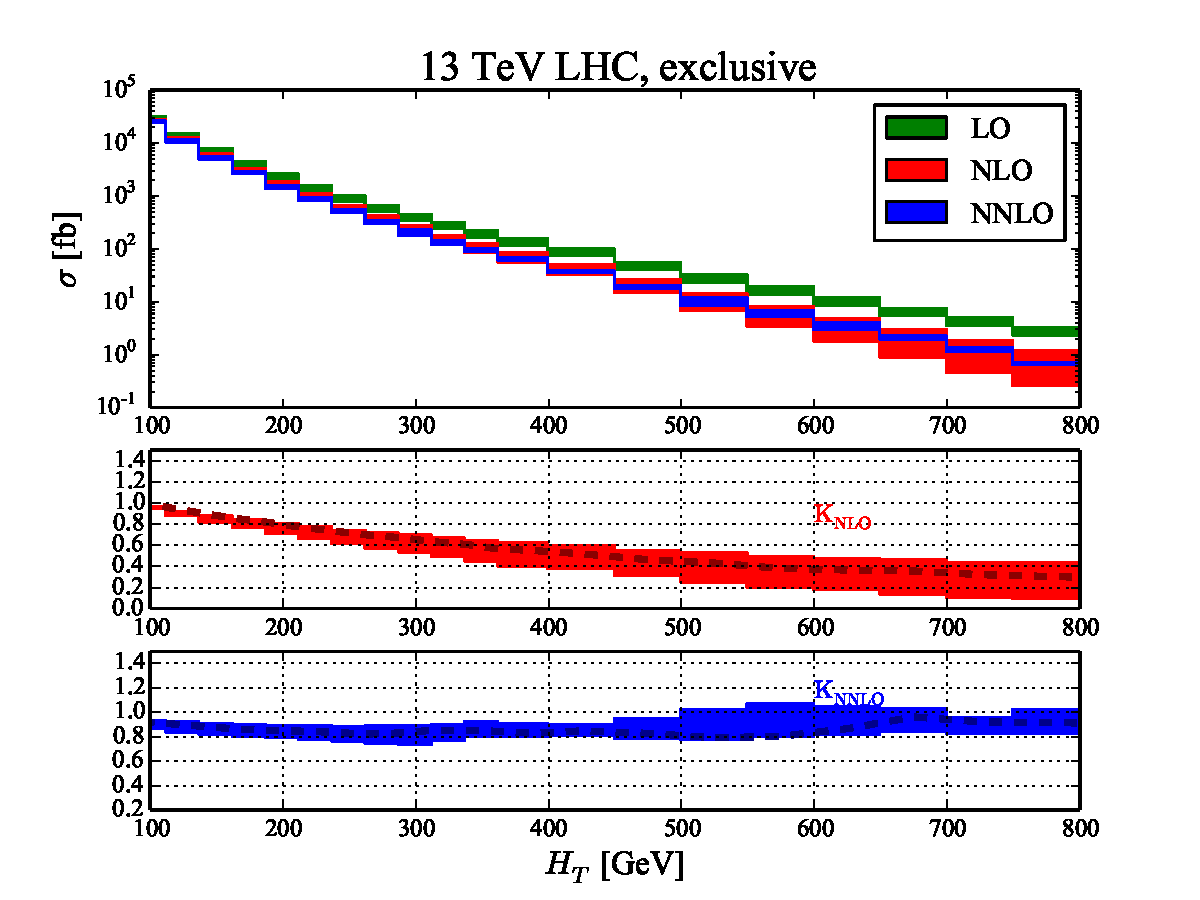
\includegraphics[width=0.495\columnwidth]{HT_13TeV_excl.pdf} 
\caption{Comparison of the NNLO \ptZ distribution normalised by the NNLO Drell-Yan cross section with data from ATLAS.}
\label{fig:ptNNLO}
\end{figure}   
Also studied is the case of the boosted W where the cut on the leading jet is required to be $> 500$ GeV. There are 2 distinct category of events that pass these selection cuts; those where the leading jet is back to back with the high pT boson and events with 2 jets with the emission of a soft or collinear W boson. The first type of eevnts occur at LO in the perturbative expansion of the W+jet process, while the second type of event first occurs at NLO. The correction in the fiducial cross section in going from the LO to NLO is large, the K-factor is 2.8 due ot this new event category that appears at NLO. The NNLO correction is smaller at 16\%and the scale variation also decreases from 20\% at NLO to less than 7\% at NNLO. The NNLO correction is contained within the NLO scale variation band, indicating convergenece of the pertubative expansion. 
The separation between the closest jet and W boson is shown in Figure. The events where the jet and W are back to back is shown in the region where $\Delta R_{j,W} > \pi$. The distribution of events in the region below this is quite broad and populaed by events where the W boson is emitted from one of the jets (a diejt configuration with the emission of a softer W boson). The NLO extends the range in $\Delta R_{j,W} > \pi$ to lower values which is influenced by dijet production with the emission of a soft W. The NNLO effects are very similar to NLO below $\pi$. Since the lepton is emitted preferentially along the W direction, the  $\Delta R_{j,l}$ distribution is similar. 

\begin{figure}[t!]
\centering
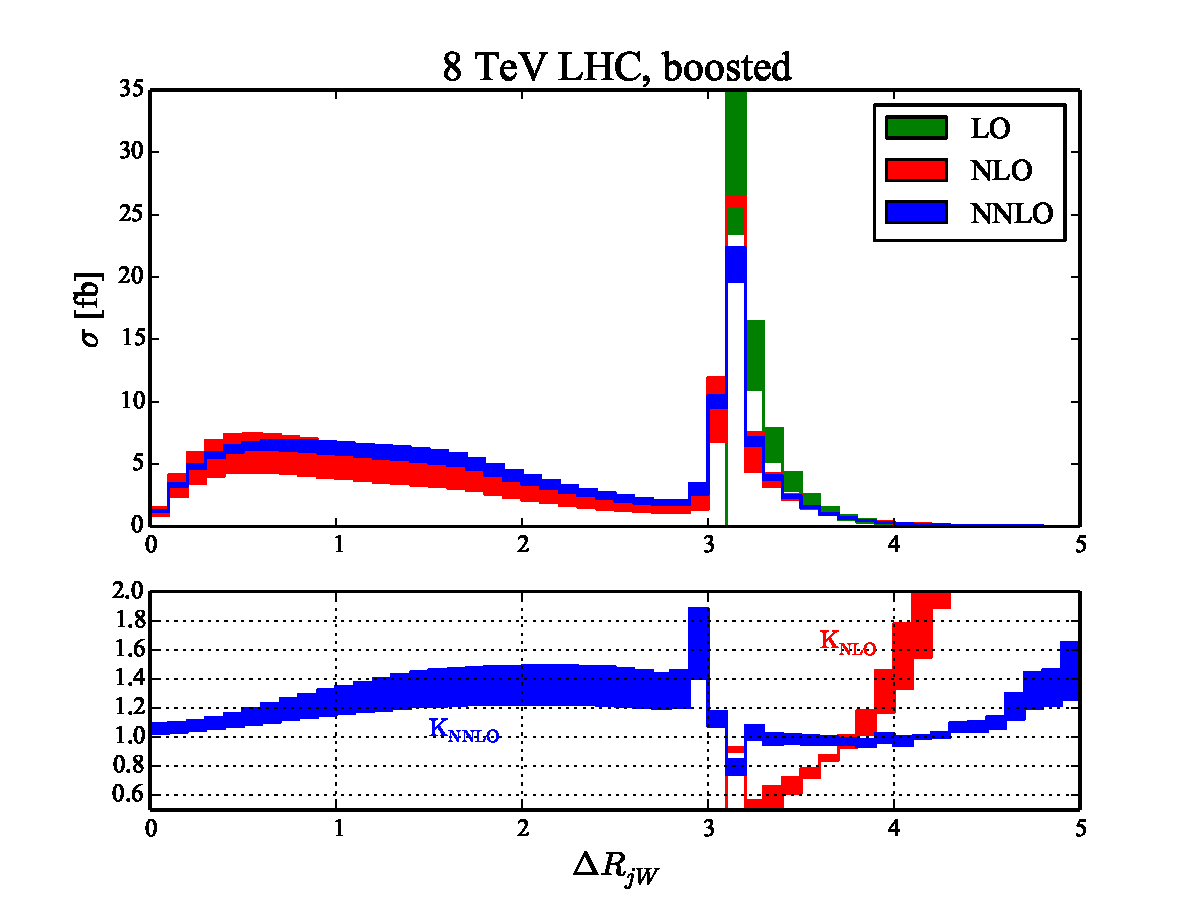
\includegraphics[width=0.495\columnwidth]{delrjW.pdf} 
\caption{Comparison of the NNLO \ptZ distribution normalised by the NNLO Drell-Yan cross section with data from ATLAS.}
\label{fig:ptNNLO}
\end{figure}   


\section{Backgrounds to BSM searches}

\section{Outcome/wishlist}
\begin{itemize}
\item V+jets crucial background in a multitude of BSM searches
Modelling of inclusive V+jets seems to be under very good control. I.e. very good MC/data agreement for various employed MCs.
\item Inclusion of EW corrections crucial in the tails of high-energy distributions: assign uncertainty to EW corrections, add Sudakov logs. Fixed EWK corrections are available in Sherpa+OpenLoops (2.2)[specify version number in results]. MC@NLO are working on it. Approximate NLO EWK corrections available in 2.2. Exact, fixed order will be available in 2.3. Recommendation being finalised for inclusive jet+MET for applying EWK corrections and uncertainties.  
\item NNLO QCD reduce scale uncertainties to the O(5\%) level for individual distributions, quantify correlations between distributions. Validate different calculations using different methods. V+jets - antenna subtraction and Njettiness slicing, validate against each other. 
\item MC/Data agreement deteriorates in more exclusive phase-space regions. In particular high-mjj (VBF). Understand the reasons for differences between generators.  
\item More exclusive distributions e.g HT in bins of Njet, 2D distributions to show correlations between variables e.g HT vs pTZ[specific?], in pTV-dphij1j2 - dijet radiates a Z - one extreme of this distribution, dijet back to back with Z other extreme, middle of this region interesting. 
\item Jet-observables \& leptonic observables if possible 
\item Where possible, unnormalized distributions, or provision of k-factor used to normalize the overall cross-section. NNLO k-factors obtained for inclusive sample (Njet >=0) not always applicable to less inclusive distributions (Njet >=1,2). Normalized in public note, unnormalized in HEPDATA?
\item Higher-order EW corrections for QCD \& EW V+jets in VBF topologies - Sherpa includes QCD corrections for VBF topologies, also EWK corrections to QCD production but not QCD corrections to EWK production. At higher order interferences between QCD and EWK production, calculate V+jets at all sub-leading one loop orders.  
\end{itemize}

\bibliography{ref}
\bibliographystyle{JHEP}

\end{document}
